\documentclass[a4paper,14pt, unknownkeysallowed]{extreport}
\usepackage{cmap} % Улучшенный поиск русских слов в полученном pdf-файле
\usepackage[T2A]{fontenc} % Поддержка русских букв
\usepackage[utf8]{inputenc} % Кодировка utf8
\usepackage[english,russian]{babel} % Языки: английский, русский
\usepackage{enumitem}


\usepackage{threeparttable}

\usepackage[14pt]{extsizes}

\usepackage{caption}
\captionsetup{labelsep=endash}
\captionsetup[figure]{name={Рисунок}}

% \usepackage{ctable}
% \captionsetup[table]{justification=raggedleft,singlelinecheck=off}

\usepackage{amsmath}

\usepackage{geometry}
\geometry{left=30mm}
\geometry{right=10mm}
\geometry{top=20mm}
\geometry{bottom=20mm}

\usepackage{titlesec}
\titleformat{\section}
{\normalsize\bfseries}
{\thesection}
{1em}{}
\titlespacing*{\chapter}{0pt}{-30pt}{8pt}
\titlespacing*{\section}{\parindent}{*4}{*4}
\titlespacing*{\subsection}{\parindent}{*4}{*4}

\usepackage{setspace}
\onehalfspacing % Полуторный интервал

\frenchspacing
\usepackage{indentfirst} % Красная строка

\usepackage{titlesec}
\titleformat{\chapter}{\LARGE\bfseries}{\thechapter}{20pt}{\LARGE\bfseries}
\titleformat{\section}{\Large\bfseries}{\thesection}{20pt}{\Large\bfseries}

\usepackage{listings}
\usepackage{xcolor}


\usepackage{pgfplots}
\usetikzlibrary{datavisualization}
\usetikzlibrary{datavisualization.formats.functions}

\usepackage{graphicx}
\newcommand{\imgScale}[3] {
	\begin{figure}[h!]
		\center{\includegraphics[scale=#1]{img/#2}} % height
		\caption{#3}
		\label{img:#2}
	\end{figure}
}

\usepackage{graphicx}
\newcommand{\imgHeight}[3] {
	\begin{figure}[h!]
		\center{\includegraphics[height=#1]{img/#2}} % height
		\caption{#3}
		\label{img:#2}
	\end{figure}
}

\usepackage[justification=centering]{caption} % Настройка подписей float объектов

\usepackage[unicode,pdftex]{hyperref} % Ссылки в pdf
\hypersetup{hidelinks}

\usepackage{csvsimple}

\newcommand{\code}[1]{\texttt{#1}}


\usepackage{longtable}

\usepackage{array}
\usepackage{booktabs}
\usepackage{floatrow}

\floatsetup[longtable]{LTcapwidth=table}


\usepackage{csvsimple}

\begin{document}
	
\renewcommand{\contentsname}{Содержание} % Переименовать table of contents
\tableofcontents
\setcounter{page}{3}

\chapter*{Введение}
\addcontentsline{toc}{chapter}{Введение}

Анализ тональности как направление компьютерной лингвистики берет начало в последней декаде XX в., и сейчас является одним из самых активно развивающихся видов автоматического анализа естественного языка \cite{Semina2}. С тех пор было выделено несколько подходов, для каждого из которых существует множество методов для решения данной задачи.

Анализ тональности находит практическое применение во многих областях: оценка качества товаров и услуг по отзывам покупателей в Интернете, анализ негативных эмоций в сообщениях, прогноз фондовых рынков, политических ситуаций на основе новостных лент. Также сентимент-анализ необходим в автоматизированных системах, в которых человек общается с машиной на естественном языке \cite{Bodrunova}. Чтобы проанализировать такой объем информации, в последние годы были предложены многочисленные методы автоматического сентимент-анализа, которые рассмотрены в данной работе.

\textbf{Целью} данной работы является исследование современных методов машинного обучения для задачи определения тональности в тексте на естественном языке.

В рамках работы необходимо решить следующие \textbf{задачи}:
\begin{itemize}
	\item рассмотреть базовые подходы к анализу тональности;
	\item рассмотреть проблемы анализа тональности;
	\item изучить существующие методы анализа тональности на основе машинного обучения;
	\item предложить критерии оценки качества методов;
	\item изучить методы решения проблем анализа тональности;
	\item выбрать метод, который наиболее эффективно решает задачу анализа тональности, учитывая проблемы этой задачи.
\end{itemize}

\chapter{Анализ предметной области}

В данном разделе обоснована актуальность задачи, представлены основные определения, базовые подходы и проблемы анализа тональности текста.

\section{Актуальность задачи}

Актуальность данной задачи обусловлена тем, что анализ тональности текста имеет широкий спектр применений в современном мире. С его помощью можно выявлять отношение пользователей к продукту, применять данный анализ для политических, социологических, экономических, маркетинговых исследований, строить рекомендательные и обучающие системы \cite{Samigulin}.

Например, современные пользовательские дискуссии в сети Интернет содержат важную социальную информацию, которую можно выявлять и изучать междисциплинарными методами. К такой информации могут относиться социальные и политические аттитюды, культурные коды, паттерны межличностного общения и распространения знаний, информация о групповых интересах и конфликтных настроениях. Картирование онлайн-дискуссий и изучение их контента имеет прогностический и антиконфликтный потенциал \cite{Bodrunova}.

\section{Основные определения}

Анализ тональности текста –- это подраздел обработки естественного языка (NLP) целью которого является классификация текста по тональности. Тональность -- это мнение, отношение и эмоции автора по отношению к объекту, о котором говорится в тексте \cite{Samigulin}. Мнение, как считает большинство исследователей в области анализа тональности, состоит из главных компонентов: субъекта (или источника), объекта (или цели) и тональности. Субъектом называется человек, которому принадлежит мнение, в ряде случаев субъектом может быть не человек, а компания или организация. Объект определяется как предмет, человек или атрибут, о котором высказано мнение \cite{Semina1}. В качестве объектов могут выступать объекты реального мира, люди, события или процессы. Обычно используется бинарная классификация, выявление в тексте положительных и отрицательных оттенков. Но также может добавляться нейтральный класс или стоять более сложная задача, допустим выявление оценок, которые поставит пользователь: «Отлично», «Хорошо», «Плохо» и другие.

Анализ тональности текстов происходит в несколько этапов \cite{Dvoinikova}:
\begin{enumerate}
	\item предобработка текста (приведение всех слов к единому регистру, удаление знаков пунктуации, удаление стоп-слов, токенизация, нормализацию слов и при необходимости иные операции);
	\item извлечение признаков (представление текста в числовом виде);
	\item классификатор (лингвистический подход, подход на основе машинного обучения, гибридный подход);
	\item оценка результата (количественная оценка результатов).
\end{enumerate}

Машинное обучение -- это методика анализа данных, которые позволяют компьютерам самостоятельно обучаться посредством решения массива сходных задач \cite{Poletaeva}. Традиционно в машинном обучении выделяют задачи обучения с учителем, обучения без учителя и с подкреплением, каждая из которых предназначена для решения конкретных проблем (рис. \ref{ml_classes}).

\begin{figure}[H]
	\centering
	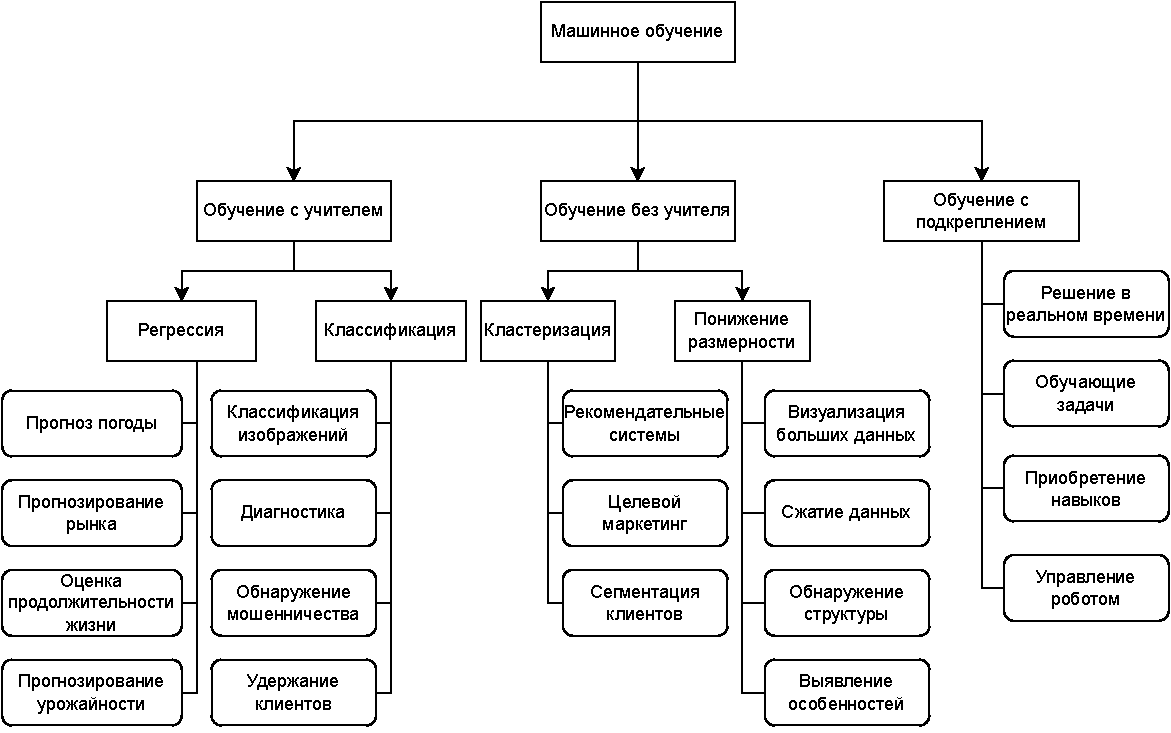
\includegraphics[scale=0.85]{imgs/ml_classes.pdf}
	\caption{Классификация и область применения систем машинного обучения}
	\label{ml_classes}
\end{figure}

В машинном обучении большое внимание уделяется автоматизированным процедурам. Другими словами, цель состоит в том, чтобы создать алгоритмы обучения, которые могут учиться самостоятельно, без необходимости взаимодействия с человеком. Машинное обучение можно рассматривать как «программирование на примере». Часто существует конкретная цель, например, проверка на спам. Вместо того, чтобы напрямую программировать компьютер для решения проблемы, машинное обучение ищет методы, позволяющие компьютеру сгенерировать свою собственную программу на основе предоставленных примеров \cite{Alhanov}.


\section{Базовые подходы к анализу тональности}

В настоящее время в основном используются следующие подходы для выявления эмоциональной окраски текста:
\begin{enumerate}
	\item лингвистический подход или анализ, основанный на правилах и словарях; 
	\item подход, основанный на использовании методов машинного обучения; 
	\item гибридный подход, сочетающий в себе подходы как на основе правил и словарей, так и на основе машинного обучения. 
\end{enumerate}	

Перечисленные методы являются стандартными для интеллектуального анализа текста, при машинном обучении анализ тональности сводится к обычной классификации.
	
	\subsection{Лингвистический подход}
	
	Данный подход основан на использовании словарей с заранее подготовленными вручную шаблонами эмоционально важных слов и словосочетаний с их эмоциональными оценками. Тональный словарь представляет собой набор слов или биграмм, которым задается определенный вес принадлежности к позитивному или негативному классу. При анализе текста каждое слово ищется в этом словаре, и его вес записывается. Если слова нет в словаре, то его класс считается нейтральным, и вес равняется нулю. После того как все веса получены, высчитывается принадлежность данного текста к определенному классу тональности. При использовании данного подхода в тексте ищутся пересечения со словарем. Затем по сумме оценок найденных пересечений определяется тональность заданного текста. Данный подход показывает хорошие результаты для некоторых областей. 
	
	Основной недостаток данного подхода заключается в большой сложности подготовки словарей, надо хорошо знать предметную область, для которой составляется словарь. Второй недостаток -- это плохая масштабируемость, нельзя использовать один и тот же словарь для разных предметных областей. Одинаковые термины в различных областях могут вносить разный вес в степень эмоциональной окраски \cite{Samigulin}.
	
	
	\subsection{Подход на основе машинного обучения}
	
	Суть данного подхода в том, что вначале на заранее размеченных данных обучается классификатор, который потом используется для классификации новых текстов. В данной работе будут подробнее рассматриваться именно методы, основанные на данном подходе \cite{Samigulin}.

	Использование алгоритмов машинного обучения для решения данных задач достаточно распространенное явление на сегодняшний день, поскольку программы, основанные на данных алгоритмах, имеют достаточно высокий показатель эффективности в сравнении с другими подходами классификации \cite{Noskov}. Обзор и сравнение алгоритмов классификации является достаточно сложной и комплексной задачей, поскольку различные входные данные могут давать разный результат. Поэтому программные реализации алгоритмов необходимо обучать и тестировать на одинаковых наборах данных.
	
	В анализе тональности широко используются только алгоритмы обучения с учителем, причем именно классификация. Это связано с особенностями регрессии и неприменимостью результатов регрессионного анализа для выявления мнений (применяется только логистическая регрессия, которая на самом деле является линейным классификатором). Обучение без учителя применяется нечасто, поскольку кластеризация, т.е. объединение документов в кластеры на основе метрик расстояния между ними, для анализа тональности редко дает хорошие результаты \cite{Semina2}.
	
	Стоит уточнить этап предобработки данных \cite{Volkova}:
	\begin{itemize}
		\item исключение стоп-слов: необходимо использовать аккуратно, т. к. некоторые стандартные стоп-слова, например, отрицательная частица <<не>> могут содержать информацию о тональности текста и удалять их не стоит;
		\item нормализация: для русского языка целесообразнее использовать лемматизацию (преобразование слова к его
		начальной форме (лемме) \cite{Dvoinikova}), а не стемминг (получение основы слова,
		при этом у слов отбрасываются окончания, суффиксы, приставки \cite{Dvoinikova}), т. к. стеммер работает менее точно;
		\item векторизация: лучшим вариантом является использование TF-IDF векторизации в сочетании с выделением N-грамм символов (чаще всего биграмм и триграмм).
	\end{itemize}
	
	\subsection{Гибридный подход}
	
	Данный подход позволяет использовать одновременно несколько подходов, например, машинное обучение может получать в качестве признаков не слова, а количество единиц, входящих в тональные лексиконы \cite{Poletaeva}. Ряд исследований показывает, что с помощью данного подхода можно добиться улучшения качества классификации, но такой подход является самым трудоемким и затратным по времени \cite{Samigulin}.


\section{Проблемы анализа тональности}

Анализ тональности, как и любой вид анализа естественного языка, имеет ряд сложно решаемых проблем.

Одной из наиболее сложных проблем считается выделение \textit{имплицитной оценки}, т. е. скрытой \cite{Semina2}. Деление мнения на имплицитное и эксплицитное типично для анализа тональности, но раньше имплицитную оценку часто опускали и не рассматривали как объект исследования из-за сложной реализации анализа. Эксплицитная оценка в тексте выражена отдельным тональным высказыванием -- словом или словосочетанием, явно выражающим тональность, это делает ее доступной для автоматического анализа. Имплицитная тональность очевидна для человека, но трудно формализуема при автоматической обработке. 

Выделение \textit{иронии и сарказма} является проблемой не только анализа тональности, но и многих других систем обработки естественного языка \cite{Semina2}. Системы обработки текста оперируют графемами и словоформами, и обучить их улавливать смысл ироничных высказываний возможно только в небольшой степени.

Анализ тональности сталкивается и с проблемами, свойственными всем видам анализа текстов, таким как необходимость
\textit{дизамбигуации} и \textit{разрешения референции} \cite{Semina2}.

Дизамбигуация или разрешение лексической многозначности далеко не всегда становится вопросом исследования, связанным с анализом тональности, но при использовании отдельных ресурсов она будет необходима. Необходимость проведения дизамбигуации связана с разной тональностью значений одного слова.

Сложность представляют и проблемы референции и кореференции. При анализе тональности для местоимений нужно устанавливать их антецеденты для верной интерпретации оценки, и неточные результаты разрешения референции могут привести к потенциальным ошибкам в анализе тональности. 

\section{Вывод}

В данном разделе была обоснована актуальность задачи, введены основные определения, рассмотрены базовые подходы к анализу тональности и проблемы анализа тональности.

\chapter{Классификация существующих решений}

В данном разделе представлены методы анализа тональности на основе машинного обучения и решения проблем, связанные с анализом тональности.

\section{Методы анализа тональности текста на основе машинного обучения}

Далее представлены основные методы традиционного машинного обучения. Дана их краткая характеристика и проанализирована их эффективность для задачи анализа тональности. 

	\subsection{Наивный байесовский классификатор}
	
	Является вероятностным классификатором. Наивная байесовская модель вычисляет условную вероятность класса на основе распределения слов в документе. Один из самых простых используемых классификаторов. Основан на теореме Байеса с предположением о том, что все признаки являются независимыми, благодаря чему и получил название наивный байесовский классификатор \cite{Samigulin}. Но обычно в текстовых документах, предположение о независимости не подтверждается, что делает его слабоэффективным. Тем не менее несмотря на всю простоту и ограничение на независимость, байесовский классификатор может показывать хорошие результаты при классификации текста. В данном исследовании с помощью наивного байесовского классификатора на различных данных получают точность от 55\% до 79\% \cite{Hasan}.
	
	Преимуществами данного метода, как было сказано, является простота реализации, малое количество данных необходимых для
	обучения, а также большая скорость работы \cite{Samigulin, Noskov}.
	
	Недостатком данного метода, как было сказано, является низкое качество классификации в большинстве случаев \cite{Samigulin}.
	
	\subsection{Метод максимума энтропии}
	
	Также как и наивный байесовский классификатор является вероятностным классификатором. Данный метод основан на принципе максимальной энтропии, что наиболее характерным распределением вероятностей неопределенной среды, являются распределения, которые максимизируют выбранную меру неопределенности при заданной информации о поведении среды. В отличии от наивного байесовского классификатора метод максимума энтропии не делает предположения о независимости признаков, что позволяет добиться лучших результатов \cite{Samigulin}. 
	
	Как и у наивного байесовского классификатора, преимуществами являются простота реализации и малое количество данных необходимых для обучения.
	
	\subsection{Деревья решений}
	
	Дерево принятия решений -- средство поддержки принятия решений, использующееся в статистике и анализе данных для прогнозных моделей. Структура дерева представляет собой «листья» и «ветки». На ребрах («ветках») дерева решения записаны атрибуты, от которых зависит целевая функция, в «листьях» записаны значения целевой функции, а в остальных узлах -- атрибуты, по которым различаются случаи. Чтобы классифицировать новый случай, надо спуститься по дереву до листа и выдать соответствующее значение. Цель состоит в том, чтобы создать модель, которая предсказывает значение целевой переменной на основе нескольких переменных на входе. Каждый лист представляет собой значение целевой переменной, измененной в ходе движения от корня по листу. Каждый внутренний узел соответствует одной из входных переменных. Дерево может быть также «изучено» разделением исходных наборов переменных на подмножества, основанные на тестировании значений атрибутов. Это процесс, который повторяется на каждом из полученных подмножеств. Рекурсия завершается тогда, когда подмножество в узле имеет те же значения целевой переменной, таким образом, оно не добавляет ценности для предсказаний \cite{Noskov}.
	
	Преимуществами данного метода являются простота в интерпретации, отсутствие требования подготовки данных, возможность работать с большим объемом информации без подготовительных процедур \cite{Samigulin, Noskov}.
	
	Недостатками данного подхода являются проблема получения оптимального дерева решений и высокая зависимость от обучающих данных. При небольших изменениях в обучающей выборке могут получиться кардинально разные результаты на тестовых данных \cite{Samigulin}.
	
	\subsection{Случайный лес}
	
	Ансамбль решающих деревьев. В данном методе строиться очень много решающих деревьев большой глубины на разных обучающих данных. Деревья строятся до тех пор, пока в каждом листе не окажется очень мало объектов, то есть они сильно переобучены. Затем все деревья объединяются и получается эффективный классификатор, у которого отсутствуют недостатки дерева решений. Но это вызывает некоторые проблемы, если признаков очень много, то этот подход работает не очень хорошо: деревья будут очень глубокими, на их построение будет уходить слишком много времени \cite{Samigulin}.
	
	Преимуществами данного метода являются все преимущества и отсутствие недостатков дерева решений.
	
	Недостатком данного метода, как было сказано, является большие временные затраты на построение глубоких деревьев с большим числом признаков \cite{Noskov}.
	
	\subsection{Логическая регрессия}
	
	Является методом линейного классификатора, оценивающий вероятность принадлежности объектов к классу путем сравнения с логической кривой по значениям множества признаков. Используется как для задач регрессии, так и для классификации. На практике часто рассматривается логическая регрессия с регуляризацией. Регуляризация заключается в том, что модель начинает штрафовать за очень большие веса, что не дает модели переобучиться. 
	
	Преимуществом данного метода является высокое качество классификации \cite{Samigulin}. 
	
	Недостатком данного подхода является необходимость качественной предобработки признаков и их отбор \cite{Noskov}.

	\subsection{Метод опорных векторов}
	
	Метод опорных векторов (SVM) -- набор линейных алгоритмов машинного обучения для задач регрессии и классификации. Цель метода заключается в нахождении среди всех возможных гиперплоскостей пространства, отделяющих два класса обучающих примеров друг от друга, такой гиперплоскости, расстояния от которой до ближайших векторов обоих классов равны (оптимальная разделяющая гиперплоскость). Является одним из наиболее эффективных методов классификации. Данный метод часто применяется в задачах классификации текстов и показывает хорошие результаты. Линейные модели хорошо масштабируются, могут работать с большим количеством признаков, на очень больших выборках \cite{Samigulin}. 
	
	На практике редко удается построить гиперплоскость, однозначно разделяющую набор данных. В наборе данных могут иметься такие документы, которые классификатор отнес к одной категории, хотя они должны принадлежать к противоположной. Такие данные создают погрешность в методе опорных векторов \cite{Noskov}.
	
	\subsection{Сравнение и оценка методов}

	На основании описанных выше методов машинного обучения для анализа тональности критерием оценки качества была выбрана высокая точность определения тональности текста.

	В исследовании методов машинного обучения в задаче автоматического определения тональности текстов на естественном языке применялись основные традиционные методы машинного обучения \cite{Samigulin}. В качестве входных данных использовались следующие англоязычные корпуса текстов:
	\begin{itemize}
		\item корпус отзывов о фильмах, входящий в состав библиотеке NLTK, 2000 текстов, в среднем 3500 символов в тексте;
		\item корпус из лексического семантического тезауруса SentiWordNet, 2000 текстов, в среднем 150 символов в тексте.
	\end{itemize}

	В качестве метрики эффективности метода использовалась AUC-площадь под ROC кривой (кривой ошибок). Авторы обучили несколько моделей, подбирая разные параметры, чтобы добиться лучших результатов. Перед этим была произведена предобработка данных и отбор признаков. Ниже представлены наилучшие результаты для различных методов традиционного машинного обучения.

	\begin{table}[H]
		\caption{Таблица результатов сравнения методов традиционного машинного обучения на основе данных из англоязычных корпусов текстов}
		
		\begin{center}
			
		\begin{tabular}{|c|c|c|}
			\hline
			Методы & Обучающая выборка & Тестовая выборка \\
			\hline
			Логическая регрессия & 0.93445 & 0.93445 \\
			\hline
			Дерево принятий решений & 0.68204 & 0.65000 \\
			\hline
			Случайный лес & 0.90799 & 0.84000 \\
			\hline
			Метод опорных векторов & 0.89416 & 0.86167 \\
			\hline
			
		\end{tabular}
			
		\end{center}
	\end{table}

	Еще одно исследование в качестве входных данных использует наборы данных содержащие отзывы о товарах с интернет-магазина \cite{Samigulin}. Метрики оценивания accuracy (точность) -- соотношение правильно предсказанных объектов к общему количеству объектов в наборе данных. В данном исследовании получились следующие результаты:

	\begin{table}[H]
		\caption{Таблица результатов сравнения методов традиционного машинного обучения на основе данных из отзывов о товарах с интернет-магазина}
		
		\begin{center}
			
			\begin{tabular}{|c|c|}
				\hline
				Методы & Точность (\%) \\
				\hline
				Метод максимума энтропии & 72.60 \\
				\hline
				Случайный лес & 88.39 \\
				\hline
				Наивный байесовский классификатор & 75.50 \\
				\hline
				Метод опорных векторов & 91.15 \\
				\hline
				
			\end{tabular}
			
		\end{center}
	\end{table}

	Как можно заметить среди методов традиционного машинного обучения наилучшие результаты показывают линейные модели: логическая регрессия и метод опорных векторов. Также неплохо себя показывает случайных лес. 

\section{Методы решения проблем анализа тональности}

Ранее были перечисленны проблемы анализа тональности, такие как:

\begin{enumerate}
	\item выделение имплицитной оценки;
	\item выделение иронии и сарказма;
	\item дизамбигуляция;
	\item разрешение референции.
\end{enumerate}

Далее представлены способы решения каждой из перечисленных проблем.

\subsection{Проблема имплицитной оценки}

Добавление списка правил можно считать одним из наиболее часто встречаемых способов улучшения работы алгоритма \cite{Semina2}. Правила могут покрывать различные виды задач.

Добавление правил может также выделить часть имплицитной информации, например, Л. Чжан и Б. Лью собрали лингвистические шаблоны для распознавания фраз, выражающих имплицитное мнение, Л. Денг и Дж. Виби использовали логические операции \cite{Semina2}. Их модель определялась использованием множества элементарных элементов или атомов и правил \textit{если -- то}, выраженных в виде правил логики первого порядка. Идея логического вывода имплицитной тональности из эксплицитной является одной из удачно формализуемых идей, поскольку создание алгоритма вывода представляется возможным.

\subsection{Проблема иронии и сарказма}

Для решения этой проблемы стоить добавить правила для поиска ироничных и саркастических конструкций, которые будут основаны на поиске фрагментов текста, соответствующих некоторому шаблону, а также определить еще один классификатор на основе машинного обучения для определения иронии и сарказма \cite{Semina2, Volkova}, помимо классификатора для анализа тональности. Классификатор тональности будет вычислять результат на основе результатов, полученные от классификатора иронии и сарказма.

Для классификатора иронии и сарказма можно также использовать метод опорных векторов или логическую регрессию. Однако предобработка данных для этого классификатора должна выполняться иначе. TF-IDF векторизация в данном случае будет неэффективной, т. к. она не учитывает связи между словами в предложении, поэтому необходимо использовать синтаксический парсер, который анализирует текст и выдает структуру зависимостей слов друг от друга в виде дерева. На основе дерева зависимойстей слов можно составить кортеж из пар слов, которые находятся в соседних узлах, причем, первым словом пары должна быть определенная часть речи (глагол, существительное или прилагательное) \cite{Volkova}.

\subsection{Проблема дизамбигуляции}

Дизамбигуляция может быть решена с помощью специальных словарей, тезаурусов, где все слова данного языка представлены максимально полно и с исчерпывающим перечнем их употребления в тексте \cite{BRE}. Для тезауруса Wordnet была проведена разметка тональности для отдельных синсетов, главных элементов этого тезауруса, и проект SentiWordnet теперь входит в библиотеку Natural Language Tool Kit \cite{Semina2}.

\subsection{Проблема референции и кореференции}

Проблема кореференции может решаться различными способами, или при помощи графа знаний, или при помощи дополнительных правил и составленных списков кореферентных элементов. Кореференция не ведет к серьезным проблемам с выделением мнений, но установление эквивалентности единиц позволит убрать дублирующиеся тональности.

\section{Вывод}

В данном разделе были представлены и сравнены методы анализа тональности на основе машинного обучения и решения проблем, связанные с анализом тональности.

\chapter*{Выводы}
\addcontentsline{toc}{chapter}{Выводы}

В рамках научно-исследовательской работы была достигнута ее цель: были изучены современные методы машинного обучения для задачи определения тональности в тексте на естественном языке. 

В результате исследования в качестве метода для анализа тональности текста был выбран метод логической регрессии как самый точный из представленных методов. Для решения проблемы имплицитной оценки был описан и выбран метод со списком правил, описывающий шаблоны имплицидных мнений. Для решения проблемы иронии и сарказма был описан и выбран метод с классификатором иронии и сарказма также на основе логической регрессии, который обучен на шаблонах ироничных и саркастических конструкций. Для решения проблемы дизамбигуляции был описан и выбран метод с использованием тезаурусов. Для решения проблемы референции и кореференции был описан и выбран метод с дополнительными правилами, т. к. это потребует лишь добавления новых правил в список правил, который уже определен для имплицитных мнений.

Также выполненны следующие задачи: 
\begin{itemize}
	\item рассмотренны базовые подходы к анализу тональности;
	\item рассмотренны проблемы анализа тональности;
	\item изучены существующие методы анализа тональности на основе машинного обучения;
	\item предложены критерии оценки качества методов;
	\item изучены методы решения проблем анализа тональности;
	\item выбран метод, который наиболее эффективно решает задачу анализа тональности, учитывая проблемы этой задачи.
\end{itemize}

Поставленная цель была достигнута.

\newpage
\addcontentsline{toc}{chapter}{Список литературы}
\renewcommand\bibname{Список литературы} % переименовать страницу списка литературы
\bibliographystyle{utf8gost705u}  % стилевой файл для оформления по ГОСТу

\begin{thebibliography}{100}
	\bibitem{Semina2} Семина Т.А. Анализ тональности текста: современные подходы и существующие проблемы [Электронный ресурс]. Режим доступа: https://cyberleninka.ru/article/n/analiz-tonalnosti-teksta-sovremennye-podhody-i-suschestvuyuschie-problemy (Дата обращения: 20.12.2021)
	
	\bibitem{Bodrunova} Бодрунова С. С. Кросс-культурный тональный анализ пользовательских текстов в Твиттере [Электронный ресурс]. Режим доступа: https://cyberleninka.ru/article/n/kross-kulturnyy-tonalnyy-analiz-polzovatelskih-tekstov-v-tvittere (Дата обращения: 20.12.2021)
	
	\bibitem{Samigulin} Самигулин Т.Р., Джурабаев А.Э.У. Анализ тональности текста методами машинного обучения [Электронный ресурс]. Режим доступа: https://cyberleninka.ru/article/n/analiz-tonalnosti-teksta-metodami-mashinnogo-obucheniya (Дата обращения: 21.12.2021)
	
	\bibitem{Semina1} Семина Т. А. Извлечение мнения автора через обратную частоту документа [Электронный ресурс]. Режим доступа: https://cyberleninka.ru/article/n/izvlechenie-mneniya-avtora-cherez-obratnuyu-chastotu-dokumenta (Дата обращения: 21.12.2021)
	
	\bibitem{Dvoinikova} Двойникова А. А., Карпов А. А. Аналитический обзор подходов к распознаванию тональности русскоязычных текстовых данных [Электронный ресурс]. Режим доступа: https://cyberleninka.ru/article/n/analiticheskiy-obzor-podhodov-k-raspoznavaniyu-tonalnosti-russkoyazychnyh-tekstovyh-dannyh (Дата обращения: 22.12.2021)
	
	\bibitem{Poletaeva} Полетаева Н.Г. Классификация систем машинного обучения [Электронный ресурс]. Режим доступа: https://cyberleninka.ru/article/n/klassifikatsiya-sistem-mashinnogo-obucheniya (Дата обращения: 22.12.2021)
	
	\bibitem{Alhanov} Алханов А. А. Машинное обучение и его применение в современном мире [Электронный ресурс]. Режим доступа: https://cyberleninka.ru/article/n/mashinnoe-obuchenie-i-ego-primenenie-v-sovremennom-mire (Дата обращения: 23.12.2021)
	
	\bibitem{Noskov} Носков Д.В. Классификация текстов при помощи алгоритмов машинного обучения [Электронный ресурс]. Режим доступа: https://cyberleninka.ru/article/n/klassifikatsiya-tekstov-pri-pomoschi-algoritmov-mashinnogo-obucheniya (Дата обращения: 24.12.2021)
	
	\bibitem{Volkova} Всероссийская студенческая конференция <<Студенческая научная весна>>, посвященная 60-летию полета Ю. А. Гагарина в космос: сборник тезисов докладов / Министерство науки и высшего образования РФ, Московский государственный технический университет им. Н. Э. Баумана, СНТО им. Н. Е. Жуковского. М.: ООО <<Издательский дом <<Научная библиотека>>, 2021, 560 с.
	
	\bibitem{Hasan} Hasan A. et al. Machine learning-based sentiment analysis for twitter accounts //Mathematical and Computational Applications. -- 2018. -- Т. 23. -- №. 1. -- P. 11.
	
	\bibitem{BRE} Большая российская энциклопедия [Электронный ресурс]. Режим доступа: https://bigenc.ru/vocabulary (Дата обращения: 26.12.2021)
	
	
\end{thebibliography}


\end{document}